\documentclass[11pt,a4paper]{scrartcl}

% ------------------------------------------------------------

% Packages
\usepackage{mathtools}
\usepackage{amssymb}
\usepackage{tikz-qtree}
\usepackage[hidelinks]{hyperref}
\usepackage{titlesec}
\usepackage{tocloft}
\usepackage[cm]{fullpage}
\usepackage{csquotes}
\usepackage{wrapfig}
\usepackage{listings}
\usepackage{xcolor}
\usepackage{makeidx}
\usepackage{ulem}

\usepackage{graphicx}
\graphicspath{{images/}}

\usepackage{parskip}
\setlength{\parindent}{0pt}

%% Packages used for symbols and signs like (c), €
\usepackage{textcomp,units}
\usepackage{enumerate}

%% Package used for nice block text
\usepackage{microtype}

\usepackage{ellipsis}
\usepackage{fixltx2e}
\usepackage{booktabs}

%% Package used for correction of wrong display 'Marginalien'
\usepackage{mparhack}

%% Package used for nicer tables
\usepackage{longtable}

%% Packages used to break long urls
\usepackage{url}
\usepackage{etoolbox}
\appto\UrlBreaks{\do\a\do\b\do\c\do\d\do\e\do\f\do\g\do\h\do\i\do\j
\do\k\do\l\do\m\do\n\do\o\do\p\do\q\do\r\do\s\do\t\do\u\do\v\do\w
\do\x\do\y\do\z}

%% Package used for German descriptions
\usepackage[ansinew]{inputenc}
\usepackage[ngerman]{babel}
\addto\captionsngerman{ 
    \renewcommand{\figurename}{Abbildung} 
    \renewcommand{\tablename}{Tabelle}
    \renewcommand{\abstractname}{Kurzfassung}
    %\renewcommand{\nomname}{Abkürzungen}
    \renewcommand{\lstlistingname}{Snippet}
    \renewcommand{\lstlistlistingname}{Verzeichnis der Snippets}
    \renewcommand{\indexname}{Stichwortverzeichnis}
}

\usepackage[automark]{scrpage2}
\automark[chapter]{chapter}
\clearscrheadfoot

% ------------------------------------------------------------

% Document Settings
%% Metadata
\title{\vspace{5cm}\huge Computer Architektur \\ \Large Studienarbeit \vspace{1cm}}
\subtitle{\Huge Emulation des Soundsystems \\ \Large Game Boy Advance Reverse Engineering \vspace{1cm}}
\author{\large \textbf{Dominik Scharnagl - Florian Boemmel - Ngoc Luu Tran}\\ \normalsize bei Nils Weis / Prof. Dr. Hackenberg}
\date{\normalsize 16. Mai 2018}

%% Language
%\selectlanguage{ngerman}

%% Colors
\definecolor{numberscolor}{RGB}{43,145,175}
\definecolor{commentcolor}{RGB}{0,128,0}
\definecolor{keywordcolor}{RGB}{0,0,255}

%% Formats
\titleformat*{\section}{\sffamily\huge\mdseries}
\titleformat*{\subsection}{\sffamily\LARGE\mdseries}
\titleformat*{\subsubsection}{\sffamily\Large\mdseries}

\def\trademark{\textsuperscript{\texttrademark}}

\lstset
{
    frame=single,
    captionpos=b,
    keepspaces=true,
    tabsize=4,
    showstringspaces=false,
    numbers=left, % display line numbers on the left
    basicstyle=\footnotesize\ttfamily,
    numberstyle=\color{numberscolor},
    commentstyle=\color{commentcolor},
    keywordstyle=\color{keywordcolor}
}

% ------------------------------------------------------------

% Commands
\renewcommand\cfttoctitlefont{\sffamily\hfill\Huge\mdseries}
\renewcommand\cftaftertoctitle{\sffamily\hfill\Large\mdseries\mbox{}}

\renewcommand{\cftsecfont}{\sffamily\Large\mdseries}
\renewcommand{\cftsubsecfont}{\sffamily\normalsize\mdseries}

\renewcommand{\cftsecpagefont}{\sffamily\Large\mdseries}
\renewcommand{\cftsubsecpagefont}{\sffamily\normalsize\mdseries}

%% Space between rows in tables
\renewcommand{\arraystretch}{1.5}

\makeindex

% ------------------------------------------------------------

\begin{document}
\sffamily

% ========== Title Page ==========
\maketitle
\thispagestyle{empty}
\clearpage

\setcounter{page}{1}

% ========== Table of Contents Page ==========

\pagenumbering{Roman}
\tableofcontents
\clearpage
\pagenumbering{arabic}

% ========== Index Page ==========

\printindex
\clearpage

% ========== Chapter 1 ==========

\section{Einleitung}

Der Game Boy Advance z\"ahlt zu einer der erfolgreichsten Spielekonsolen der Welt. Der 2001 von Nintendo\cite{NintendoGeschichte} ver\"offentlichte Nachfolger des Game Boy Classic findet sich heute noch in den Schubl\"aden der damalilgen Jugend. Deshalb \"uberrascht es auch nicht, dass die Fans der Konsole den Erinnerungen aus ihrer Kindheit neues Leben einhauchen und sogar Emulatoren f\"ur diverse Spiele-Klassiker der Plattform entwickeln.

\begin{figure}[h]
    \centering
    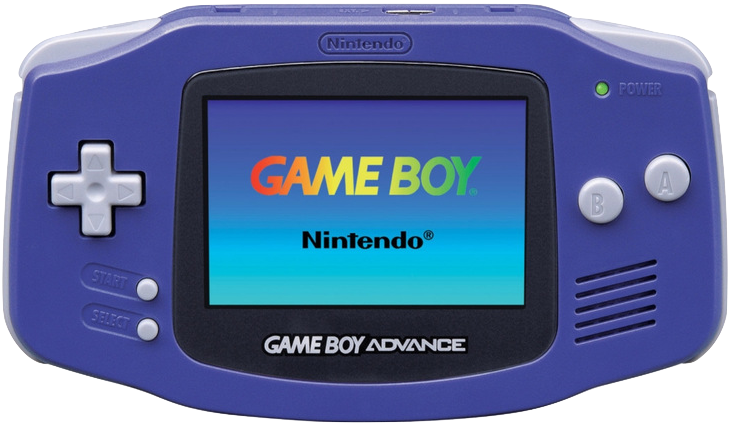
\includegraphics[width=0.5\textwidth]{GameBoyAdvance}
    \caption{Game Boy Advanced - Blue Edition}
    \label{fig:gba}
\end{figure}

Der zentrale Inhalt der Studienarbeit, ist das Reverse Engineering eines solchen Game Boy Advance Emulators. Der genaue Inhalt dieser wird in den n\"achsten Kapiteln zun\"achst eingeschr\"ankt und sp\"ater weiter konkretisiert.

Emulatoren geh\"oren zu einem beliebten Werkzeug der Informatik. Sie bilden ein System oder ein Teilsystem ab. Dabei ist zu beachten, dass diese nur bekanntes Verhalten nur \enquote{nachahmen}. Genauer ausgef\"uhrt bedeutet dies, dass zum Beispiel bei einem Game Boy Advance Emulator die Software intern anders als auf dem originalen Ger\"at arbeitet. Jedoch kommt es beim Emulieren nicht auf die gleiche Arbeitsweise an, sondern auf das Ergebnis. In diesem konkreten Fall, einen voll funktionsf\"ahigen Nachbau des Game Boys in Software. Mit dem es m\"oglich ist digitalisierte Versionen eines Spieles spielen zu k\"onnen.\newline

\begin{table}[h]
    \centering
    \begin{tabular}{ r | p{10cm} }
        \textbf{CPU} & 16,77 MHz 32 Bit RISC (ARM7TDMI)\newline
              8 Bit CISC CPU (Z80/8080-Derivat) \\
        \hline
        \textbf{Arbeitsspeicher} & 32 KB IRAM (1 cycle/32 bit)\newline
                          + 96 KB VRAM (1-2 cycles)\newline
                          + 256 KB ERAM (6 cycles/32 bit) \\
        \hline
        \textbf{Lautsprecher} & Lautsprecher (Mono), Kopfh\"orer (Stereo) \\
    \end{tabular}
    \caption{Technische Daten des Game Boy Advance\cite{GameBoyTechnischeDaten}}
    \label{table:TechnischeDaten}
\end{table}

\newpage

\subsection{Untersuchungsgegenstand}

In dieser Studienarbeit wird die Fragestellung, wie wird das Soundsystem des Game Boy Advance in einem beliebigen Emulator emuliert, thematisiert. Ein konkreter Emulator wurde nicht vorgegeben. Wir einigten uns demnach auf den Game Boy Advance Emulator \enquote{mgba}. Dieser stellt im Folgenden unseren zentralen Untersuchungsgegenstand dar.

Die Untersuchung wird in vier Unterthemen gegliedert:

\begin{itemize}
    \item Erstellung eines Beispielprogramms
    \item Untersuchung der Fragestellung mit Hilfe eines Beispielprogrammes
    \item Untersuchung der Interaktion des Beispielprogrammes mit dem Emulator
    \item Untersuchung der Interaktion von Emulator und Betriebssystem
\end{itemize}

\subsection{Verwendete Software}

\begin{itemize}
    \item \textbf{Betriebssysteme}: Ubuntu 16.0 x64, Windows 10 x64, macOS 10.13.4
    \item \textbf{Disassembler}: IDA Pro
    \item \textbf{Emualtor}: mGBA
    \item \textbf{SDK}: devkitPro
    \item \textbf{IDE's}: Programmer's Notepad, Visual Studio Code, Eclipse, Qt Creator
\end{itemize}


% ========== Chapter 2 ==========

\section{Emulation des Soundsystems}

Der Game Boy Advance verf\"ugt \"uber sechs Soundkan\"ale. Vier davon wurden, vor allem aus Gr\"unden der Abw\"artskompatibilit\"at, aus dem Vorg\"anger \enquote{Game Boy Classic} \"ubernommen.

\begin{table}[h]
    \centering
    \begin{tabular}{ r | p{10cm} }
        \textbf{Kanal} & \textbf{Art} \\
        \hline
        1 & Rechteckwellengenerator (square wave generator) \\
        \hline
        2 & Rechteckwellengenerator (square wave generator) \\
        \hline
        3 & Klangerzeuger (Sample-Player) \\
        \hline
        4 & Rauschgenerator (Noise-Generator) \\
        \hline
        A & Direct Sound \\
        \hline
        B & Direct Sound \\
    \end{tabular}
    \caption{\"Ubersicht der Soundkan\"ale des Game Boy Advance}
    \label{table:TechnischeDaten}
\end{table}

Intern besitzt der Game Boy Advance drei Sound-Master-Register. Dort m\"ussen, je nach Einstellungswunsch, ein paar Bits gesetzt werden. Erst dann ist eine Soundwiedergabe oder die generelle Funktionsf\"ahigkeit des Soundsystems m\"oglich.\cite{GameBoySoundsystem}

% ========== Chapter 2.1 ==========

\subsection{\"Ubersicht der Register}

Der Offset im Folgenden bezieht sich auf die Basisadresse $0x04000000$ und wird in hexadezimaler Schreibweise angegeben. An dieser Stelle muss darauf hingewiesen werden, dass die Bezeichnungen der Register nicht eindeutig sind und sich je nach verwendeter Quelle unterscheiden.

\begin{table}[h]
    \centering
    \begin{tabular}{ c | c | p{10cm} | l }
        \textbf{Offset} & \textbf{Kanal} & \textbf{Funktion} & \textbf{Bezeichnung} \\
        \hline
        $0x060$ & 1 & DMG Sweep control & \verb|SOUND1CNT_L| \\
        \hline
        $0x062$ & 1 & DMG Length, wave and evelope control & \verb|SOUND1CNT_H| \\
        \hline
        $0x064$ & 1 & DMG Frequency, reset and loop control & \verb|SOUND1CNT_X| \\
        \hline
        $0x068$ & 2 & DMG Length, wave and evelope control & \verb|SOUND2CNT_L| \\
        \hline
        $0x06C$ & 2 & DMG Frequency, reset and loop control & \verb|SOUND2CNT_H| \\
        \hline
        $0x070$ & 3 & DMG Enable and wave ram bank control & \verb|SOUND3CNT_L| \\
        \hline
        $0x072$ & 3 & DMG Sound length and output level control & \verb|SOUND3CNT_H| \\
        \hline
        $0x074$ & 4 & DMG Frequency, reset and loop control & \verb|SOUND3CNT_X| \\
        \hline
        $0x078$ & 4 & DMG Length, output level and evelope control & \verb|SOUND4CNT_L| \\
        \hline
        $0x07C$ & 4 & DMG Noise parameters, reset and loop control & \verb|SOUND4CNT_H| \\
        \hline
        $0x080$ & & DMG Master Control & \verb|SOUNDCNT_L| \\
        \hline
        $0x082$ & & Direct Sound Master Control & \verb|SOUNDCNT_H| \\
        \hline
        $0x084$ & & Master Sound Output Control / Status & \verb|SOUNDCNT_X| \\
        \hline
        $0x088$ & & Sound Bias & \verb|SOUNDBIAS| \\
        \hline
        $0x090 - 0x09F$ & 3 & DMG Wave RAM Register & \verb|WAVERAM0-3| \\
        \hline
        $0x0A0 - 0x0A2$ & A & Direct Sound FIFO & \verb|FIFO_A| \\
        \hline
        $0x0A4 - 0x0A6$ & B & Direct Sound FIFO & \verb|FIFO_B| \\
    \end{tabular}
    \caption{\"Ubersicht der Sound-Register}
    \label{table:SoundRegister}
\end{table}
\newpage

% ========== Chapter 2.2 ==========

\subsection{\"Ubersicht der Register des Sound Masters}

Die Register DMG Master Control, Direct Sound Master Control und Master Sound Output Control / Status bilden die Sound Master Register.\\

% ========== Chapter 2.2.1 ==========

\subsubsection{DMG Master Control} \label{dmgmastercontrol}

	Hier m\"ussen zun\"achst einige Bits gesetzt werden, bevor eine generelle Verwendung des Sound-Systems m\"oglich ist.\\

	\begin{table}[h]
	\centering
	\begin{tabular}{| c | c | c | c | c | c | c | c | c | c | c | c |}
	\hline
	F & E & D & C & B & A & 9 & 8 & 7 & 6 5 4 & 3 & 2 1 0 \\
	\hline
	\textcolor{blue}{R4} & \textcolor{blue}{R3} & \textcolor{blue}{R2} & \textcolor{blue}{R1} & \textcolor{red}{L4} & \textcolor{red}{L3}
	& \textcolor{red}{L2} & \textcolor{red}{L1} & - & \textcolor{magenta}{RV} & - & \textcolor{green}{LV} \\
	\hline
	
	\end{tabular}
	\caption{Register DMG Master Control}
	\label{table: DMGMasterControl}
	\end{table}
	
	\begin{table}[h]
	\centering
	\begin{tabular}{| c | c | c | c |}
	\hline
	\textbf{Bits} & \textbf{Name} & \textbf{Definition} & \textbf{Beschreibung} \\
	\hline
	0-2 & \textcolor{green}{LV} & & Left volume \\
	\hline
	4-6 & \textcolor{magenta}{RV} & & Right volume \\
	\hline
	8-B & \textcolor{red}{L1-L4} & SDMG\_LSQR1,  & Channels 1-4 on left \\
	& & SDMG\_LSQR2, & \\
	& & SDMG\_LWAVE, & \\
	& & SDMG\_LNOISE & \\
  \hline
	C-F & \textcolor{blue}{R1-R4} & SDMG\_RSQR1, & Channels 1-4 on right \\
	& & SDMG\_RSQR2, & \\
	& & SDMG\_RWAVE, & \\
	& & SDMG\_RNOISE & \\
	\hline
	
	\end{tabular}
	\caption{Registerinhalt DMG Master Control}
	\label{table: DMGMasterControlContent}
	\end{table}

\newpage

% ========== Chapter 2.2.2 ==========

\subsubsection{Direct Sound Master Control}

	Dieses Register kontrolliert die Lautst\"arke der DMG Kan\"ale und aktiviert diese. Die Einstellungen k\"onnen separiert voneinander f\"ur den linken und rechten Lautsprecher vorgenommen werden. 

	\begin{table}[h]
	\centering
	\begin{tabular}{| c | c | c | c | c | c | c | c | c | c | c | c |}
	\hline
	F & E & D & C & B & A & 9 & 8 & 7 6 5 4 & 3 & 2 & 1 0 \\
	\hline
	\textcolor{brown}{BF} & \textcolor{magenta}{BT} & \textcolor{green}{BL} & \textcolor{green}{BR} & \textcolor{brown}{AF} & \textcolor{magenta}{AT}
	& \textcolor{green}{AL} & \textcolor{green}{AR} & - & \textcolor{blue}{BV} & \textcolor{blue}{AV} & \textcolor{red}{DMGV} \\
	\hline
	
	\end{tabular}
	\caption{Register Direct Sound Master Control}
	\label{table: DirectSoundMasterControl}
	\end{table}
	
	\begin{table}[h]
	\centering
	\begin{tabular}{| c | l | l | l |}
	\hline
	\textbf{Bits} & \textbf{Name} & \textbf{Definition} & \textbf{Beschreibung} \\
	\hline
	0-1 & \textcolor{red}{DMGV} & SDS\_DMG25, & DMG Volume ratio \\
	& & SDS\_DMG50, & 00: 25\% \\
	& & SDS\_DMG100 & 01: 50\% \\
	& & & 10: 100\% \\
  & & & 11: forbidden \\
	\hline
	2 & \textcolor{blue}{AV} & SDS\_A50, SDS\_A100 & DSound A volume ratio. 50\% if clear; 100\% of set  \\
	\hline
	3 & \textcolor{blue}{BV} & SDS\_B50, SDS\_B100 & DSound B volume ratio. 50\% if clear; 100\% of set  \\
	\hline
	8-9 & \textcolor{green}{AR,AL} & SDS\_AR, SDS\_AL & DSound A enable Enable DS A on right and left speakers \\
	\hline
	A & \textcolor{magenta}{AT} & SDS\_ATMR0, & Dsound A timer. Use timer 0 (if clear) or 1 (if set) for DS A \\
	& & SDS\_ATMR1 & \\
	\hline
	B & \textcolor{brown}{AF} & SDS\_ARESET &  FIFO reset for Dsound A. When using DMA for Direct sound,  \\
	& & & this will cause DMA to reset the FIFO buffer after it's used.\\
	\hline
	C-F & \textcolor{green}{BR, BL},  &  SDS\_BR, SDS\_BL, & As bits 8-B, but for DSound B \\
	& \textcolor{magenta}{BT}, \textcolor{brown}{BF} & SDS\_BTMR0,  & \\
	& & SDS\_BTMR1, & \\
	& &  SDS\_BRESET & \\
	\hline
	\end{tabular}
	\caption{Registerinhalt Direct Sound Master Control}
	\label{table: DirectSoundMasterControlContent}
	\end{table}
	
	\newpage
	
	% ========== Chapter 2.2.3 ==========
	
\subsubsection{Master Sound Output Control / Status}
	
	Aus diesem Register kann zu einem der Status der einzelnen DMG Kan\"ale ausgelesen werden und zum Anderen die generelle Soundausgabe aktiviert werden. Dazu muss das Bit 7 gesetzt werden.
	
	\begin{table}[h]
	\centering
	\begin{tabular}{| c | c | c | c | c | c | c |}
	\hline
	F E D C B A 9 8 & 7 & 6 5 4 & \textcolor{red}{3} & \textcolor{red}{2} & \textcolor{red}{1} & \textcolor{red}{0} \\
	\hline
	- & \textcolor{red}{MSE} & - & \textcolor{blue}{4A} & \textcolor{blue}{3A} & \textcolor{blue}{2A} & \textcolor{blue}{1A} \\
	\hline
	
	\end{tabular}
	\caption{Register Master Sound Output / Status}
	\label{table: MasterSoundOutputStatus}
	\end{table}
	
	\begin{table}[h]
	\centering
	\begin{tabular}{| c | l | l | l |}
	\hline
	\textbf{Bits} & \textbf{Name} & \textbf{Definition} & \textbf{Beschreibung} \\
	\hline
	\textcolor{red}{0-3} & \textcolor{blue}{1A-4A} & SSTAT\_SQR1, & Active channels. Indicates which DMA channels are currently playing.   \\
	& & SSTAT\_SQR2, & They do not enable the channels;\\
	& & SSTAT\_WAVE, & that's what DMG Master Control \ref{dmgmastercontrol} is for.\\
	& & SSTAT\_NOISE & \\
	\hline
	7 & \textcolor{red}{MSE} & SSTAT\_DISABLE, & Master Sound Enable. Must be set if any sound is to be heard at all.   \\
	& & SSTAT\_ENABLE & Set this before you do anything else: \\
	& & & the other registers can't be accessed otherwise, see GBATek for details. \\ 
	\hline
	\end{tabular}
	\caption{Registerinhalt Master Sound Output / Status}
	\label{table: MasterSoundOutputStatusContent}
	\end{table}

\clearpage

\subsection{Interaktion mit dem Betriebssystem}

\begin{figure}[h]
    \centering
    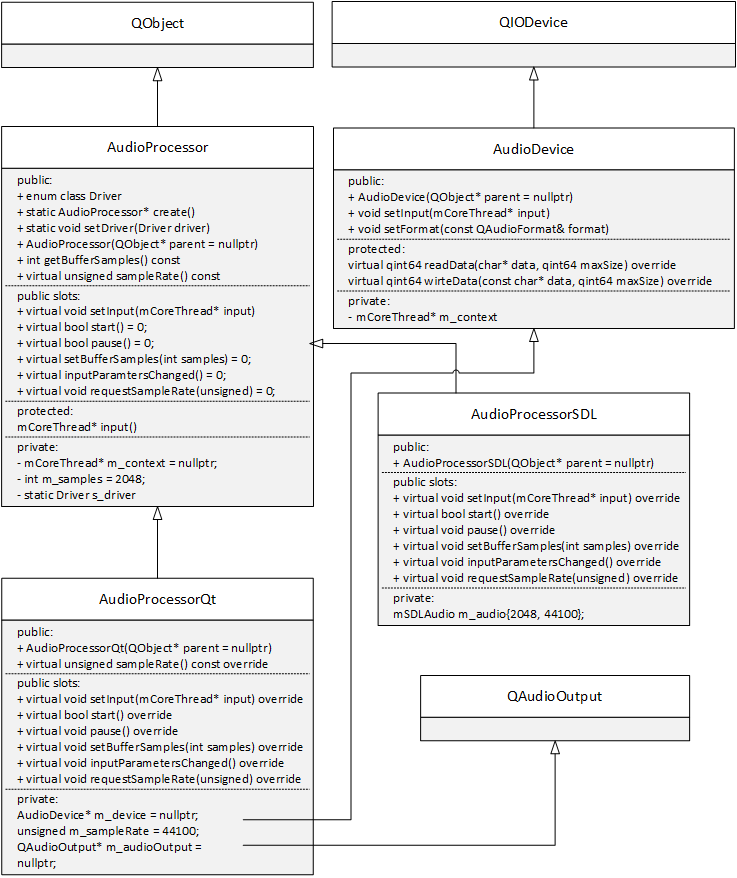
\includegraphics[width=0.7\textwidth]{QT_Klassendiagramm}
    \caption{Audioklassen in der QT-Anwendung}
    \label{fig:qtclassdiagramm}
\end{figure}


\addtocontents{toc}{\protect\setcounter{tocdepth}{-1}}

\begin{thebibliography}{tiefe}
    \bibitem{NintendoGeschichte}Nintendo: \textit{Game Boy Advance}\newline
    \url{https://www.nintendo.de/Unternehmen/Unternehmensgeschichte/Game-Boy-Advance/Game-Boy-Advance-627139.html}, Mai 2018
    \bibitem{GigaEmulator}Giga Ratgeber: \textit{Was ist der Unterschied zwischen Simulation, Emulation \& Virtualisierung?}\newline
    \url{https://www.giga.de/extra/ratgeber/specials/was-ist-der-unterschied-zwischen-simulation-emulation-virtualisierung-computertechnik/}, Mai 2018
    \bibitem{GameBoyTechnischeDaten}Nintendo: \textit{Game Boy Advance}\newline
    \url{http://de.nintendo.wikia.com/wiki/Game_Boy_Advance}, Mai 2018
    \bibitem{GameBoySoundsystem}Coranac: \textit{18. Beep! GBA sound introduction}\newline
    \url{https://www.coranac.com/tonc/text/sndsqr.htm#sec-intro}, Mai 2018
\end{thebibliography}

\vspace{1cm}

\huge Bilder
\normalsize

\begin{itemize}
    \item Abbildung \ref{fig:gba}: \textit{Game Boy Advance - Blue Edition}\newline
    \url{https://d3nevzfk7ii3be.cloudfront.net/igi/L3WryntCMswfDks1.large}, Mai 2018
\end{itemize}
\end{document}











